\documentclass[twoside, ngerman, draft]{sdqthesis}

\author{Ilia Chupakhin}

\title{Extrahieren von Code-Änderungen aus einem Commit für kontinuierliche Integration von Leistungsmodellen}

\thesistype{Codereview für eine Bachelorarbeit}

\reviewerone{Prof. Dr.-Ing. Anne Koziolek}
\reviewertwo{Prof. Dr. Ralf H. Reussner}

\advisorone{M.Sc. Manar Mazkatli}
%\advisortwo{???}

%\editingtime{24. Juli 2020}
\date{24. Juli 2020}
\settitle


\hyphenation{
}

%\usepackage{listings}
%\usepackage{color}


\usepackage[citestyle=numeric,style=numeric,hyperref,backend=biber]{biblatex}
\usepackage{hyperref}
\addbibresource{sections/Literatur.bib}


\begin{document}

\setpdf

\maketitle

\frontmatter

%
\thispagestyle{empty}
\null\vfill
\noindent\hbox to \textwidth{\hrulefill} 
\iflanguage{english}{I declare that I have developed and written the enclosed
thesis completely by myself, and have not used sources or means without
declaration in the text.}%
{Ich versichere wahrheitsgemäß, die Arbeit
selbstständig angefertigt, alle benutzten Hilfsmittel vollständig und genau
angegeben und alles kenntlich gemacht zu haben, was aus Arbeiten anderer
unverändert oder mit Änderungen entnommen wurde.}
 
 


\textbf{Ort, Datum}
\vspace{1.5cm}
 
\dotfill\hspace*{8.0cm}\\
\hspace*{2cm}(\theauthor) 
\cleardoublepage

\setcounter{page}{1}
\pagenumbering{roman}

\tableofcontents

\mainmatter

\chapter{Einleitung}
\label{ch:Einleitung}

Ein Performance-Modell ermöglicht den Software-Entwicklern eine frühzeitige Analyse von programmierten Komponenten in Bezug auf Leistungseigenschaften, wie zum Beispiel Speicherbedarf oder Ausführungsdauer. Das Performance-Modell muss mit allen anderen im System vorhandenen Modellen konsistent gehalten werden. Falls ein Modell geändert wurde, muss auch das Performance-Modell aktualisiert werden. Allerdings ist eine Aktualisierung des Performance-Modells für große Systeme aufwändig. Ein Ansatz für eine effiziente Aktualisierung von Performance-Modellen wurde in \cite{mazkatli2018} vorgestellt und in \cite{mazkatli2020} weiterentwickelt. Wir bezeichnen diesen Ansatz als Continuos Integration of Performance Model (CIPM). 
\\
In dieser Bachelorarbeit implementieren wir den ersten Schritt für den CIPM-Ansatz. Wir verknüpfen den CIPM-Ansatz mit einem Git Repository und extrahieren Änderungen aus Commits. Anhand von den extrahierten Änderungen passen wir die existierenden Code-Modelle an. Anschließend werden diese Änderungen zu den Performance-Modellen automatisch propagiert. Für diesen Zweck haben wir die existierenden Change-Propagation-Regeln angepasst und einige neue Regeln implementiert.
\\ 
Unsere Implementierung haben wir in einer Case-Study evaluiert. Für ein Projekt haben wir unterschiedliche Arten von Änderungen simuliert und sie als Commits in einem Git-Repository gespeichert. Danach haben wir dieses Projekt in Vitruvius integriert, Änderungen aus den Commits gelesen und die entsprechenden Modelle angepasst. Anschließend haben wir die Korrektheit der aktualisierten Code- und Performance-Modelle überprüft.
\\
Das Kapitel \ref{ch:Installationsanleitung} enthält eine Installationsanleitung und Instruktionen für die Ausführung von Tests. In dem Kapitel \ref{ch:Architektur} beschreiben wir die Architektur unserer Implementierung und der dazu gehörenden Tests. Die Ergebnisse der durchgeführten Case-Study zeigen wir in dem Kapitel \ref{ch:Case-Study-Ergebnisse}.

\chapter{Installationsanleitung}
\label{ch:Installationsanleitung}


\section{Software-Installation}
\label{sec:Software-Installation}
\begin{itemize}
\item Java, Version 12 
\item Eclipse Modeling Tools, Version 2020-03 \\\href{https://www.eclipse.org/downloads/packages/release/2020-03/r}{https://www.eclipse.org/downloads/packages/release/2020-03/r}
\item In Eclipse im Menü "Help -> Install new software" die folgenden Plugins installieren:
	\begin{itemize}
	\item Henshin\\\href{http://download.eclipse.org/modeling/emft/henshin/updates/release}{http://download.eclipse.org/modeling/emft/henshin/updates/release} 
	\item EMFText, Version 1.4.1 \\\href{http://update.emftext.org/trunk/}{http://update.emftext.org/trunk/}
	\item JaMoPP, Version 1.4.1 \\\href{http://update.jamopp.org/trunk/}{http://update.jamopp.org/trunk/}	
	\item Palladio, Version 4.1 (release 1.1.0) \\\href{https://updatesite.palladio-simulator.com/palladio-build-updatesite/releases/1.1.0/}{https://updatesite.palladio-simulator.com/palladio-build-updatesite/releases/1.1.0/}
	\item Vitruvius \\\href{https://vitruv-tools.github.io/updatesite/nightly/}{https://vitruv-tools.github.io/updatesite/nightly/}
	\item SoMoX \\\href{http://kit-sdq.github.io/updatesite/nightly/somox/jamopp/}{http://kit-sdq.github.io/updatesite/nightly/somox/jamopp/}
	\end{itemize}
\item Die folgenden Plugins von \href{https://github.com/vitruv-tools/Vitruv-Applications-PCMJavaAdditionals}{https://github.com/vitruv-tools/Vitruv-Applications-PCMJavaAdditionals} von dem Branch "modelsUpdateFromGitCommits"  herunterladen und in Eclipse workspace importieren (File -> Import -> General -> Existing Projects into Workspace):
	\begin{itemize}
	\item org.palladiosimulator.pcm.modified
	\item org.somox.test.gast2seff
	\item tools.vitruv.applications.pcmjava.integrationFromGit
	\item tools.vitruv.applications.pcmjava.integrationFromGit.test
	\item tools.vitruv.applications.pcmjava.linkingintegration
	\item tools.vitruv.applications.pcmjava.linkingintegration.change2command
	\item tools.vitruv.applications.pcmjava.linkingintegration.ejbtransformations
	\item tools.vitruv.applications.pcmjava.seffstatements
	\item tools.vitruv.applications.pcmjava.seffstatements.pojotransformations
	\end{itemize}
\item Alle Plugins von \href{https://github.com/maxil063/sdq/tree/master/changedPlugins}{https://github.com/maxil063/sdq/tree/master/changedPlugins} von dem Branch "master"  herunterladen und in Eclipse workspace importieren (File -> Import -> General -> Existing Projects into Workspace).
\end{itemize}

\section{Ausführung von Tests}
\label{sec:Ausführung von Tests}
In Eclipse Run Configuration öffnen (Run -> Run Configuration). In der Liste 'JUnit Plug-in Test' das Plugin tools.vitruv.applications.pcmjava.integrationFromGit.test wählen. Es wird empfohlen, die Tests einzeln auszuführen. 'Run a single test' aktivieren, als 'Test Class' einen Test aus der Liste wählen (Die Namen von den ausführbaren Tests fangen mit 'IA' oder mit 'NIA' an), als 'Test runner' JUnit 4 wählen und die Option 'Run in UI Thread' deaktivieren (das ermöglicht eine Interaktion mit dem Benutzer mithilfe von User Dialogs).  
\\
Während der Ausführung wird in manchen Tests ein User Dialog mehrmals gezeigt, wo der Benutzer eine Wahl treffen muss. Falls der Benutzer keine Wahl trifft, wird der Test nach dem zweiten Timeout weiter ausgeführt und liefert falsche Ergebnisse oder schlägt fehl. Die folgenden Wahlmöglichkeiten werden zur Zeit unterstützt:
\begin{itemize}
\item 'create Basic Component' falls ein Package oder eine Klasse erstellt wurde
\item 'create interface' falls ein Interface erstellt wurde
\end{itemize}
In manchen Tests werden Timeouts ausgelöst, obwohl es kein User Dialog angezeigt wurde. In diesem Fall wird der Test nach zwei Timeouts weiter korrekt ausgeführt. 
 

\chapter{Architektur}
\label{ch:Architektur}
Unsere Implementierung ist in dem Plugin tools.vitruv.applications.pcmjava.integrationFromGit. Die Tests befinden sich in dem Plugin\\ tools.vitruv.applications.pcmjava.integrationFromGit.test. Die unvollständigen Klassendiagramme für die beiden Plugins sind in den Abbildungen \ref{fig:integrationFromGit} und \ref{fig:integrationFromGit_test} dargestellt.

\begin{figure}[h]
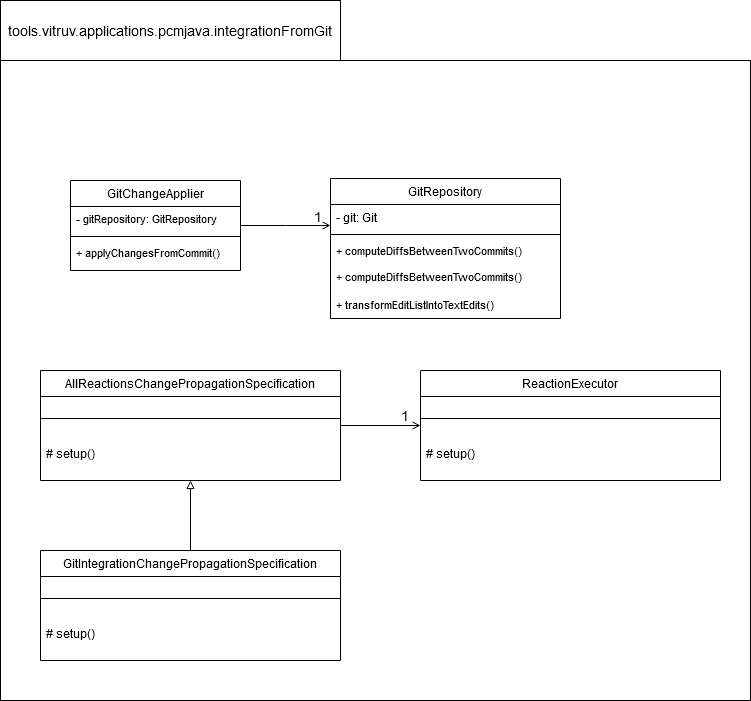
\includegraphics[width=\textwidth]{pictures/integrationFromGit_diagram.png}
\caption{Klassendiagram für das Plugin tools.vitruv.applications.pcmjava.integrationFromGit. Das Klassendiagramm ist unvollständig und dient nur einer Darstellung der einzelnen Klassen, Methoden und Variablen.}
\label{fig:integrationFromGit}
\end{figure}

\begin{figure}[h]
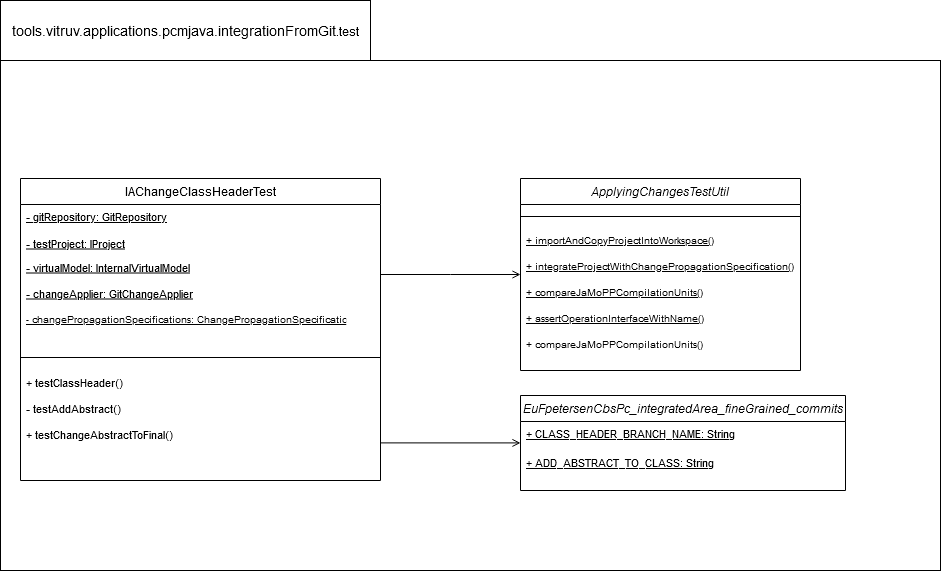
\includegraphics[width=\textwidth]{pictures/integrationFromGitTest_diagram.png}
\caption{Klassendiagram für das Plugin tools.vitruv.applications.pcmjava.integrationFromGit.test. Das Klassendiagramm ist unvollständig und dient nur einer Darstellung der einzelnen Klassen, Methoden und Variablen.}
\label{fig:integrationFromGit_test}
\end{figure}

\section{Plugin tools.vitruv.applications.pcmjava.integrationFromGit}

Die Klasse GitChangeApplier wendet extrahierte Änderungen auf die Code-Modelle an. Die Hauptmethode applyChangesFromCommit nimmt als Parameter zwei Commits, zwischen denen Änderungen ausgerechnet werden müssen, sowie ein JDT-Modell von einem Java-Projekt. Die Methode ermittelt Änderungen, klassifiziert sie und ruft eine passende Routine auf. Zum Beispiel, für eine als 'ADD' klassifizierte Änderung wird die Methode addElementToProject aufgerufen. Nach einer erfolgreichen Ausführung sind die Änderungen auf das JDT-Modell von dem Java-Projekt angewandt. Falls dieses Projekt in Vitruvius integriert ist, werden auch die JaMoPP-Modelle in VSUM automatisch angepasst und gegebenenfalls auch die korrespondierenden PCM-Modelle.
\\ 
Anders als in dem GitChangeReplay-Tool \footnote{GitChangeReplay-Tool: https://github.com/vitruv-tools/GitChangeReplay} werden in unserer Implementierung die aus einem Commit extrahierten Änderungen nicht in atomare Änderungen zerlegt. Für unseren Zweck ist es nicht notwendig. Darüber hinaus würde das die Performance unserer Implementierung negativ beeinträchtigen.
\\
Änderungen an den JaMoPP-Modellen in VSUM werden von dem Monitor detektiert. Anschließend werden die entsprechenden Listener benachrichtigt. Dieser Mechanismus ermöglicht eine Aktualisierung von den korrespondierenden Performance-Modellen. Als Performance-Modelle haben wir die Palladio Component Models (PCM) benutzt. Um die Performance-Modelle automatisch anpassen zu können, muss eine Change Propagation Specification (CPS) und Change Propagation Rules (CPR) definiert werden. Unsere CPS ist in der Klasse GitIntegrationChangePropagationSpecification definiert. Die CPR haben wir in der Reaction-Sprache definiert. Sie befinden sich in den Dateien PackageAndClassifiers.reactions und ClassifierBody.reactions. Die meisten CPR haben wir aus den folgenden Projekten übernommen und angepasst:

\begin{itemize}
\item \begin{scriptsize}
tools.vitruv.applications.pcmjava.linkingintegration.change2command.internal.response.PackageMappingIntegration.reactions\end{scriptsize}
\item tools.vitruv.applications.pcmjava.pojotransformations.java2pcm
\end{itemize}

Die CPR für die Änderungen innerhalb der Methoden haben wir unverändert gelassen. Sie stammen aus dem folgenden Projekt:
\begin{itemize}
\item \begin{scriptsize}tools.vitruv.applications.pcmjava.seffstatements.pojotransformations.Java2PcmPackageMappingMethodBodyChangePreprocessor.xtend
\end{scriptsize}\end{itemize}

Außerdem haben wir auch neue CPR definiert. Zum Beispiel eine Reaktion auf löschen einer Klasse und eines Packages. Die Anpassungen in den bereits existierenden CPR waren notwendig, weil sie für unsere Case-Study nicht (korrekt) funktioniert haben. Ein Grund dafür war, dass die ursprünglichen CPR nicht für die integrierten Projekte gedacht sind, sondern für die Projekte, die von Anfang an mit Vitruvius entwickelt wurden. Zum Beispiel, wenn ein neues Package erstellt wurde, wurden automatisch  Subpackages 'datatypes' und 'contracts' erstellt. Das hat aber zu Inkonsistenzen zwischen der Projektstruktur in dem Git Repository und der in Vitruvius geführt, weil in Git Repository keine Subpackages 'datatypes' und 'contracts' existieren.

\section{Plugin tools.vitruv.applications.pcmjava.integrationFromGit.test}

Die Tests haben wir in zwei Packages unterteilt:

\begin{itemize}
\item tools.vitruv.applications.pcmjava.integrationFromGit.test.integratedArea
\item tools.vitruv.applications.pcmjava.integrationFromGit.test.nonIntegratedArea
\end{itemize}

Die Tests in tools.vitruv.applications.pcmjava.integrationFromGit.test.integratedArea simulieren Änderungen auf den Teilen des Projekts, die bereits vor der Integration in Vitruv existiert haben und als einen integrierten Bereich zählen. Was als ein integrierter Bereich zählt ist projektspezifisch. In unserem Test-Projekt gelten alle Packages innerhalb des source-Packages als integrierten Bereich. Mehr Details über integrierte und nicht integrierte Bereiche können in \cite{langhammer2017} gefunden werden. Die Tests in\\ tools.vitruv.applications.pcmjava.integrationFromGit.test.integratedArea simulieren Änderungen auf den Teilen des Projekts, die vor der Integration in Vitruv noch nicht existiert haben. Außerdem finden diese Änderungen in einem Bereich statt, der als nicht integrierten Bereich zählt. In unserem Test-Projekt zählt ein neues Package innerhalb des source-Packages als ein nicht integrierter Bereich. Das neue Package darf nicht in die anderen schon existierenden Subpackages verschachtelt sein. Sonst würde es als ein integrierter Bereich erkannt.
\\
In unseren Tests wollten wir zeigen, dass die von uns angepassten Change Propagation Rules (CPR) sich gleich verhalten ungeachtet darauf, ob Änderungen in einem integrierten oder nicht integrierten Bereich stattgefunden haben. In der Zukunft sollte diese Unterscheidung komplett irrelevant sein, weil der CIPM-Ansatz \cite{mazkatli2018} auf den Java-Projekten mit beliebigen Strukturen anwendbar sein soll.
\\
In dem Package tools.vitruv.applications.pcmjava.integrationFromGit.test.commits sind die Namen von den Git-Branches und Commit-Hashes für alle Tests gespeichert.
\\
In dem Ordner tools.vitruv.applications.pcmjava.integrationFromGit.test/testProjects ist unser Test-Projekt gespeichert.
\\
In der Klasse ApplyingChangesTestUtil.java sind die Hilfsmethoden für alle Tests enthalten. Die meisten Methoden sind statisch und können deshalb auch in den anderen Projekten benutzt werden.
\\
Jeder Test überprüft die Korrektheit unserer Implementierung für einen bestimmten Änderungstypen. Zum Beispiel der Test IAChangeClassHeaderTest.java simuliert Änderungen eines Klassenkopfes. Das Präfix 'IA' steht für Integrated Area und 'NIA' für Non-Integrated Area. Alle Tests haben eine ähnliche Struktur:
\\
1. Vorbereitung (setUpBeforeClass-Methode):
\\
Zuerst wird ein Projekt in das aktuelle Workspace kopiert und ein JDT-Modell davon erstellt (IProject testProject). Ebenso wird dieses Projekt mit seinem Git-Repository in das Workspace kopiert (in einen separaten Ordner namens 'clonedGitRepositories'). Die Objekte GitRepository und GitChangeApplier verweisen auf 'clonedGitRepositories'. Das erstellte JDT-Modell (IProject testProject) wird in Vitruvius integriert. Dabei entsteht ein Ordner 'vitruvius.meta' in dem Workspace, ein Monitor, der Änderungen zu den korrespondierenden Modellen propagiert, und ein InternalVirtualModel-Objekt. Das InternalVirtualModel-Objekt enthält unter anderem eine Referenz auf die 'vitruvius.meta'-Ordner und\\GitIntegrationChangePropagationSpecification-Objekt. Für die Tests in den nicht integrierten Bereichen werden auch nicht integrierte Bereiche vorbereitet (Packages, Klassen, Interfaces erstellt).
\\
2. Der eigentliche Test:
\\
Die Abbildung \ref{fig:method} zeigt einen Test für das Hinzufügen einer Klassenvariable in einer Klasse, die in einem integrierten Bereich liegt. Zuerst wird eine Änderung  aus einem Commit gelesen und auf das in Vitruvius integrierte Projekt angewandt (changeApplier.applyChangesFromCommit(...)) und das geänderte JDT-Modell gefunden (ICompilationUnit compUnitChanged). Als Referenzmodell wird das Git-Repository an dem gleichen Commit ausgecheckt und ein temporäres JDT-Modell von der gleichen (aber nicht der selben) Compilation Unit erstellt (gitRepository.checkoutFromCommitId(...) und ICompilationUnit compUnitFromGit). Anschließend werden die JaMoPP-Modelle für die beiden Compilation Units (compUnitChanged und compUnitFromGit) verglichen (ApplyingChangesTestUtil.compareJaMoPPCompilationUnits(...)). Das JaMoPP-Modell für compUnitFromGit wird neu erstellt während das JaMoPP-Modell für compUnitChanged wird aus InternalVirtualModel genommen. Als letztes wird es überprüft, ob ein PCM-Modell für die neu erstellte Klassenvariable existiert (ApplyingChangesTestUtil.assertFieldWithName(...)). Eine explizite Überprüfung der nötigen Korrespondenz ist nicht notwendig, weil sie implizit in der Methode ApplyingChangesTestUtil.assertFieldWithName(...) stattfindet.
\begin{figure}[h]
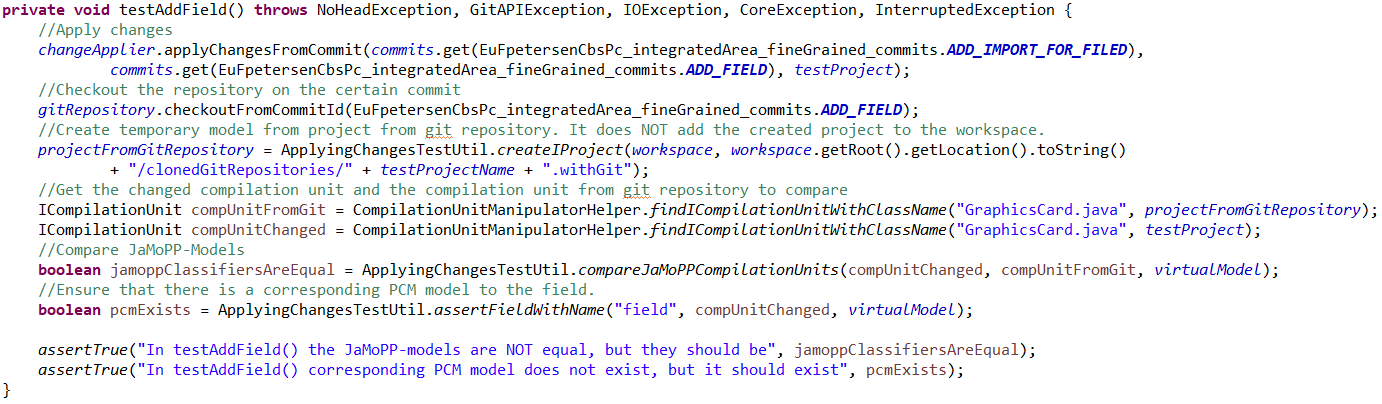
\includegraphics[width=\textwidth]{pictures/method_example.png}
\caption{Test für das Hinzufügen einer Klassenvariable in einer Klasse, die in einem integrierten Bereich liegt}
\label{fig:method}
\end{figure}
\chapter{Case-Study-Ergebnisse}
\label{ch:Case-Study-Ergebnisse}
Für unsere Case-Study haben wir das Projekt namens 'eu.fpetersen.cbs.pc' \footnote{\href{https://github.com/vitruv-tools/Vitruv-Applications-PCMJavaAdditionals/tree/master/tests/tools.vitruv.applications.pcmjava.linkingintegration.tests/example_code/eu.fpetersen.cbs.pc}{eu.fpetersen.cbs.pc}} benutzt. Für dieses Projekt haben wir ein Git Repository initialisiert und Commits für unterschiedliche Arten von Änderungen erstellt. Anschließend haben wir das Projekt in Vitruvius integriert, Commits auf dem integrierten Projekt angewandt und die Korrektheit von den aktualisierten Modellen überprüft. Die Ergebnisse sind in der Tabelle \ref{tab:casestudy} abgebildet.


\begin{tiny}
%\resizebox{\textwidth}{!}{
% Please add the following required packages to your document preamble:
% \usepackage{longtable}
% Note: It may be necessary to compile the document several times to get a multi-page table to line up properly

%\setlength\LTleft{0pt}
%\setlength\LTright{0pt}
%\begin{longtable}[c]{@{\extracolsep{\fill}}|p{3cm}|p{3cm}|p{2cm}|%p{2cm}|p{2cm}|p{4cm}|}



\begin{longtable}[c]{|p{2.2cm}|p{3.5cm}|p{1cm}|p{1cm}|p{1cm}|p{4cm}|}

%\scriptsize
%\begin{tabularx}{\textwidth}{XXX}
\hline
Test & Subtests & JaMoPP Codebuffer & JaMoPP Modelle & PCM Modelle & Probleme \\ \hline
\endhead
%
testClassAnnotation 			(IA) & testAddClassAnnotation & korrekt & korrekt & nicht 			betroffen &  \\ \hline
 & testChangeClassAnnotation & korrekt & korrekt & nicht 			betroffen &  \\ \hline
 & testRemoveClassAnnotation & korrekt & korrekt & nicht 			betroffen &  \\ \hline
testClassHeader 			(IA) & testAddAbstract & korrekt & korrekt & nicht 			betroffen &  \\ \hline
 & testChangeAbstractToFinal & korrekt & korrekt & nicht 			betroffen &  \\ \hline
 & testRenameClass & nicht 			überprüft & nicht 			überprüft & nicht 			überprüft & Vitruv throws an exception when a class is removed. Because rename class is considered as remove class with old name and create class with new name, that test fails. In tools.vitruv.domains.java.monitorededitor. ChangeResponder.visit(DeleteClassEvent) the visit(...) method tries to get some information from the already removed JDT model. \\ \hline
testExtends (IA) & testAddImport & korrekt & korrekt & nicht 			betroffen &  \\ \hline
 & testAddExtends & korrekt & korrekt & keine 			CPR implementiert &  \\ \hline
 & testRemoveExtends & korrekt & korrekt & keine 			CPR implementiert &  \\ \hline
testChangeField 			(IA) & testAddImport & korrekt & korrekt & nicht 			betroffen &  \\ \hline
 & testAddField & korrekt & korrekt & korrekt &  \\ \hline
 & testRenameField & korrekt & korrekt & korrekt &  \\ \hline
 & testAddFieldModifier & korrekt & korrekt & nicht 			betroffen &  \\ \hline
 & testChangeFieldModifier & korrekt & korrekt & nicht 			betroffen &  \\ \hline
 & testChangeFieldType & korrekt & nicht korrekt  & nicht überprüft & ChangeFieldTypeEventRoutine does not work appropriate \\ \hline
 & testRemoveField & nicht 			überprüft & nicht 			überprüft & nicht 			überprüft & remove 			field event is recognized as InsertEReference, but not as 			RemoveEReference. \\ \hline
testImplements 			(IA) & testAddImport & korrekt & korrekt & korrekt &  \\ \hline
 & testAddImplements & korrekt & korrekt & korrekt &  \\ \hline
 & testRemoveImplements & korrekt & korrekt & korrekt &  \\ \hline
testChangeMethodHeader 			(IA) & testRenameMethodInInterface & korrekt & korrekt & korrekt &  \\ \hline
 & testRenameMethodInClass & korrekt & korrekt & korrekt &  \\ \hline
 & testChangeReturnTypeInInterfaceMethod & korrekt & korrekt & korrekt &  \\ \hline
 & testChangeReturnTypeInClassMethod & korrekt & korrekt & nicht 			betroffen &  \\ \hline
 & testAddReturn0InClassMethod & korrekt & korrekt & nicht 			betroffen &  \\ \hline
 & testAddFinalModifierToClassMethod & korrekt & korrekt & nicht 			betroffen &  \\ \hline
 & testAddMethodParameterInInterface & korrekt & korrekt & korrekt &  \\ \hline
 & testAddMethodParameterInClass & korrekt & korrekt & nicht 			betroffen &  \\ \hline
testChangeMethod- Implementation 			(IA) & testAddInternalAction & korrekt & korrekt & korrekt &  \\ \hline
 & testAddForLoop & korrekt & korrekt & korrekt &  \\ \hline
 & testAddIfElse & korrekt & korrekt & korrekt &  \\ \hline
 & testRemoveIfElse & korrekt & korrekt & korrekt &  \\ \hline
 & testRemoveForLoop & korrekt & korrekt & korrekt &  \\ \hline
 & testRemoveInternalAction & korrekt & korrekt & korrekt &  \\ \hline
testCreateDelete- NonJavaFile 			(IA) & testCreateFolderAndFile & nicht 			betroffen & nicht 			betroffen & nicht 			betroffen &  \\ \hline
 & testRenameFile & nicht 			betroffen & nicht 			betroffen & nicht 			betroffen &  \\ \hline
 & testChangeFileContent & File-Inhalt 			korrekt & nicht 			betroffen & nicht 			betroffen &  \\ \hline
 & testCopyFile & File-Inhalt 			korrekt & nicht 			betroffen & nicht 			betroffen &  \\ \hline
 & testRemoveFile & nicht 			betroffen & nicht 			betroffen & nicht 			betroffen &  \\ \hline
testCreateDelete- CompilationUnit 			(IA) & testCreateClass & korrekt & korrekt & korrekt &  \\ \hline
 & testCreateInterface & korrekt & korrekt & korrekt &  \\ \hline
 & testRemoveClass & nicht 			überprüft & nicht 			überprüft & nicht 			überprüft & testRemoveClass() and testRemoveInterface() doesn't work appropriate. The problem could be in the method tools.vitruv.domains.java.monitorededitor. ChangeResponder.visit(DeleteClassEvent) and tools.vitruv.domains.java.monitorededitor. ChangeResponder.visit(DeleteInterfaceEvent). The method visit(...) tries to get some information from the already removed JDT model. \\ \hline
 & testRemoveInterface & nicht 			überprüft & nicht 			überprüft & nicht 			überprüft & The 			same problem as discribed above \\ \hline
testCreateDeleteField 			(IA) & testAddImport & korrekt & korrekt & nicht 			betroffen &  \\ \hline
 & testAddField & korrekt & korrekt & korrekt &  \\ \hline
 & testRenameField & korrekt & korrekt & korrekt &  \\ \hline
 & testRemoveCreatedField & nicht 			überprüft & nicht 			überprüft & nicht 			überprüft & Somehow remove field event is recognized by Vitruv as InsertEReference, but not as RemoveEReference. Therefore, a wrong correspondence is created \\ \hline
 & testRemoveIntegratedField &  &  &  & The same problem as discribed above \\ \hline
testCreateDeleteMethod 			(IA) & testCreateMethodInInterface & korrekt & korrekt & korrekt &  \\ \hline
 & testCreateMethodInClass & korrekt & korrekt & korrekt &  \\ \hline
 & testRemoveMethodInClass & korrekt & korrekt & korrekt &  \\ \hline
 & testRemoveMethodInInterface & korrekt & korrekt & korrekt &  \\ \hline
testCreateDeletePackage 			(IA) & testCreatePackage & korrekt & korrekt & korrekt &  \\ \hline
 & testRenameCreatedPackage & korrekt & korrekt & korrekt &  \\ \hline
 & testRemoveCreatedPackage & korrekt & korrekt & korrekt &  \\ \hline
testClassAnnotation 			(NIA) & testAddClassAnnotation & korrekt & korrekt & nicht 			betroffen &  \\ \hline
 & testChangeClassAnnotation & korrekt & korrekt & nicht 			betroffen &  \\ \hline
 & testRemoveClassAnnotation & korrekt & korrekt & nicht 			betroffen &  \\ \hline
testClassHeader 			(NIA) & testRemovePublicClassModifier & korrekt & korrekt & nicht 			betroffen &  \\ \hline
 & testAddFinalClassModifier & korrekt & korrekt & nicht 			betroffen &  \\ \hline
 & testChangeFinalToAbstractClassModifier & korrekt & korrekt & nicht 			betroffen &  \\ \hline
 & testChangeAbstractToPublicClassModifier & korrekt & korrekt & nicht 			betroffen &  \\ \hline
testExtends 			(NIA) & testAddFirstImportForExtends & korrekt & korrekt & nicht 			betroffen &  \\ \hline
 & testAddExtends & korrekt & korrekt & keine 			CPR implementiert &  \\ \hline
 & testAddSecondImportForExtends & korrekt & korrekt & nicht 			betroffen &  \\ \hline
 & testChangeExtends & korrekt & korrekt & keine 			CPR implementiert &  \\ \hline
 & testRemoveExtends & korrekt & korrekt & keine 			CPR implementiert &  \\ \hline
 & testRemoveSecondImportForExtends & korrekt & korrekt & nicht 			betroffen &  \\ \hline
 & testRemoveFirstImportForExtends & korrekt & korrekt & nicht 			betroffen &  \\ \hline
testField 			(NIA) & testAddSecondClassForField & korrekt & korrekt & korrekt &  \\ \hline
 & testAddImportForField & korrekt & korrekt & nicht 			betroffen &  \\ \hline
 & testAddField & korrekt & korrekt & Nicht 			korrekt, kein PCM-Field erstellt & Die 			Klasse SecondClass hat kein korrespondierendes Interface =\textgreater in 			der Methode  			mir.routines.classifierBody.FieldCreated-CorrespondingToRepositoryComponent-Routine.ActionUserExecution.callRoutine1 (Classifier, 			Field, RepositoryComponent, RepositoryComponent, RoutinesFacade) 			werden keine operationProvidedRoles 			gefunden =\textgreater keine OperationRequiredRole wird ertellt \\ \hline
 & testRenameField & korrekt &  &  &  \\ \hline
 & testRemoveField & korrekt &  &  &  \\ \hline
 & testRemoveImportForField & korrekt &  &  &  \\ \hline
testImplements 			(NIA) & testAddFirstInterface & korrekt & korrekt & korrekt &  \\ \hline
 & testAddMethodInFirstInterface & korrekt & korrekt & korrekt &  \\ \hline
 & testAddFirstImport & korrekt & korrekt & nicht 			betroffen &  \\ \hline
 & testAddImplementsAndMethod & korrekt & korrekt & korrekt &  \\ \hline
 & testAddSecondInterface & korrekt & korrekt & korrekt &  \\ \hline
 & testAddMethodInSecondInterface & korrekt & korrekt & korrekt &  \\ \hline
 & testAddSecondImport & korrekt & korrekt & nicht 			betroffen &  \\ \hline
 & testChangeImplementsAndAddMethod & korrekt & korrekt & korrekt &  \\ \hline
 & testRemoveImplements & korrekt & korrekt & korrekt &  \\ \hline
 & testRemoveBothMethods & korrekt & korrekt & korrekt &  \\ \hline
 & testRemoveBothImports & korrekt & korrekt & nicht 			betroffen &  \\ \hline
testChangeMethodHeader 			(NIA) & testRenameMethodInInterface & korrekt & korrekt & korrekt &  \\ \hline
 & testRenameMethodInClass & korrekt & korrekt & korrekt &  \\ \hline
 & testChangeReturnTypeInInterfaceMethod & korrekt & korrekt & korrekt &  \\ \hline
 & testChangeReturnTypeInClassMethod & korrekt & korrekt & nicht 			betroffen &  \\ \hline
 & testAddReturn0InClassMethod & korrekt & korrekt & nicht 			betroffen &  \\ \hline
 & testAddFinalModifierToClassMethod & korrekt & korrekt & nicht 			betroffen &  \\ \hline
 & testAddMethodParameterInInterface & korrekt & korrekt & korrekt &  \\ \hline
 & testAddMethodParameterInClass & korrekt & korrekt & nicht 			betroffen &  \\ \hline
testMethodImplementation 			(NIA) & testAddFirstInternalAction & korrekt & korrekt & korrekt &  \\ \hline
 & testAddImport & korrekt & nicht 			korrekt &  &  \\ \hline
 & testAddFirstExternalAction & korrekt &  &  &  \\ \hline
 & testAddSecondInternalActionAndLoop WithSecondExternalAction & korrekt &  &  &  \\ \hline
 & testAddIfElseWithInternalAction AndExternalCall & korrekt &  &  &  \\ \hline
\caption{Ergebnisse der Case-Study. Abkürzungen: IA - Integrated Area, NIA - Non-Integrated Area, CPR - Change Propagation Rules.}
\label{tab:casestudy}\\
\end{longtable}

%} 
 
\end{tiny} 
 
%Probleme:
%\\
%Synchronisation : 
%EqualityHelper
%Zugriff auf Korrespondenzen
%Lösung: in manchen Tests Thread.sleep(5000)
%
%Kein OpenSource Projekt
%
%Kein Projekt mit einem existierenden VSUM
%
%Extract nicht ausführbar. Darüber hinaus, das benutzt JaMoPP
%
%SoMoX nicht ausführbar in Java 12
%
%JaMoPP problematisch
%
%Vitruv does not react to add/change/remove class annotation
%
%//testRenameClass() is disabled by now: Vitruv throws an exception when a class is removed. Because rename class 
%//is considered as remove class with old name and create class with new name, that test fails.
%//The problem could be in the method tools.vitruv.domains.java.monitorededitor.ChangeResponder.visit(DeleteClassEvent)
%//visit(...) method tries to get some information from the already removed JDT model.
%	
%	
%//Vitruv does not react to add/change/remove super class 
%
%//ChangeFieldTypeEventRoutine does not work appropriate
%//testChangeFieldType();
%//RemovedFieldEventRoutine can't find the field because of previous test testChangeFieldType().
%//Second problem: somehow remove field event is recognized as InsertEReference, but not as RemoveEReference.
%//testRemoveField();
%
%
%//testRemoveClass() and testRemoveInterface() doesn't work appropriate.
%//The problem could be in the method tools.vitruv.domains.java.monitorededitor.ChangeResponder.visit(DeleteClassEvent) 
%//and tools.vitruv.domains.java.monitorededitor.ChangeResponder.visit(DeleteInterfaceEvent) 
%//visit(...) method tries to get some information from the already removed JDT model.
%	
%//remove field doesn't work appropriate.
%//problem: somehow remove field event is recognized by Vitruv as InsertEReference, but not as RemoveEReference.
%//Therefore, a wrong correspondence is created



\printbibliography[heading=bibintoc]

\end{document}
